% author: Simon Bachmann

\section{Smart Contracts}\label{sec:smart_cont:eval}

At the time of writing this evaluation (30th of October 2020), the current gas prices is 34 Gwei for average transaction speed and 1 ETH is worth 380 USD. For all the analysis these values are used.

\subsection{Gas Cost Analysis}\label{subsection:gas-cost-analysis}

\subsubsection{Deployment of the Smart Contracts}

A factory pattern is applied in this project. The factory is responsible to create new events and to keep track of already created events. This contract is lightweight but it imports the event contract which holds most of the functionality. The \textit{EventFactory} contract must only be deployed once. 

The contracts are built in a way that the entire event specific functionality is maintained in the \textit{Event} contract. Deploying a new instance of a SC is expensive. Section \ref{subsection:gas-cost-analysis} shows this in more detail. Thus, combining all the functionality for managing fungible as well as non fungible ticket types in one contract results in lower gas costs for the event host. 

\begin{table}[ht]
\centering
\begin{tabular}{|c|c|c|c|c|}
\hline
\textbf{Contract} & \textbf{Contract Size {[}kb{]}} & \textbf{Gas Used} & \textbf{Price ETH} & \textbf{Price USD} \\ \hline
IdetixLibrary     & 0.39                         & 139370            & 0.005              & 1.80               \\ \hline
Identity          & 1.17                         & 311961            & 0.011              & 4.03               \\ \hline
EventFactory      & 23.93                       & 5367566           & 0.182              & 69.34              \\ \hline
Event             & 21.61                        & 4756013           & 0.162              & 61.45              \\ \hline
\end{tabular}
\caption{Gas cost analysis of smart contracts}
\label{tab:gas-cost-analysis-sc}
\end{table}

\subsubsection{Transactions}
The SCs are designed such that the number of on-chain transactions can be kept as low as possible. Since signing a transaction always results in a media break between the application and the wallet, the SCs favour less but expensive transactions over many cheap transactions. As an example, the event host can create multiple ticket types in one transaction. Table \ref{tab:gas-cost-ticket-types} illustrates how the gas prices behave if multiple ticket types are created in one transactions. Table \ref{tab:gas-cost-buying-ticket-types} show how the gas prices evolve if multiple tickets are bought within the same transaction. In this scenario, one affiliate is included in the transaction to make the price estimations more realistic.

\begin{table}[ht]
\centering
\begin{tabular}{|c|c|c|c|c|c|}
\hline
{ \textbf{\begin{tabular}[c]{@{}c@{}}\#Fungible\\ Types\end{tabular}}} & { \textbf{\begin{tabular}[c]{@{}c@{}}\#NF \\ Types\end{tabular}}} & { \textbf{\begin{tabular}[c]{@{}c@{}}Gas \\ Used\end{tabular}}} & { \textbf{\begin{tabular}[c]{@{}c@{}}Price \\ ETH\end{tabular}}} & { \textbf{\begin{tabular}[c]{@{}c@{}}Price \\ USD\end{tabular}}} & { \textbf{\begin{tabular}[c]{@{}c@{}}Price USD \\ per Ticket Type\end{tabular}}} \\ \hline
{ 1}                                                                    & { 0}                                                               & { 115656}                                                       & { 0.0039}              & { 1.49}                                                          & { 1.49}                                                                          \\ \hline
{ 2}                                                                    & { 0}                                                               & { 184088}                                                       & { 0.0062}                                                        & { 2.37}                                                          & { 1.19}                                                                          \\ \hline
{ 10}                                                                   & { 0}                                                               & { 731625}                                                       & { 0.0248}                                                        & { 9.45}                                                          & { 0.94}                                                                          \\ \hline
{ 0}                                                                    & { 1}                                                               & { 115690}                                                       & { 0.0039}                                                        & { 1.49}                                                          & { 1.94}                                                                          \\ \hline
{ 1}                                                                    & { 1}                                                               & { 203322}                                                       & { 0.0069}                                                        & { 2.63}                                                          & { 1.32}                                                                          \\ \hline
{ 10}                                                                   & { 10}                                                              & { 819345}                                                       & { 0.0278}                                                        & { 10.59}                                                         & { 1.05}                                                                          \\ \hline
\end{tabular}                    
\caption{Gas cost analysis for creating ticket types within one transaction}
\label{tab:gas-cost-ticket-types}
\end{table}


\begin{table}[ht]
\centering
\begin{tabular}{|c|c|c|c|c|c|}
\hline
{ \textbf{\begin{tabular}[c]{@{}c@{}}\#Fungible\\ Tickets\end{tabular}}} & { \textbf{\begin{tabular}[c]{@{}c@{}}\#NF \\ Tickets\end{tabular}}} & { \textbf{\begin{tabular}[c]{@{}c@{}}Gas \\ Used\end{tabular}}} & { \textbf{\begin{tabular}[c]{@{}c@{}}Price \\ ETH\end{tabular}}} & { \textbf{\begin{tabular}[c]{@{}c@{}}Price \\ USD\end{tabular}}} & { \textbf{\begin{tabular}[c]{@{}c@{}}Price USD \\ per Ticket\end{tabular}}} \\ \hline
{ 1}                                                                    & { 0}                                                               & { 117328}                                                       & { 0.0040}              & { 1.52}                                                          & { 1.52}                                                                          \\ \hline
{ 2}                                                                    & { 0}                                                               & { 117328}                                                       & { 0.0040}                                                        & { 1.52}                                                          & { 0.76}                                                                          \\ \hline
{ 10}                                                                   & { 0}                                                               & { 117328}                                                       & { 0.0040}                                                        & { 1.52}                                                          & { 0.15}                                                                          \\ \hline
{ 0}                                                                    & { 1}                                                               & { 145383}                                                       & { 0.0049}                                                        & { 1.88}                                                          & { 1.88}                                                                          \\ \hline
{ 0}                                                                    & { 2}                                                               & { 179586}                                                       & { 0.0061}                                                        & { 2.32}                                                          & { 1.16}                                                                          \\ \hline
{ 0}                                                                    & { 10}                                                              & { 453240}                                                       & { 0.0154}                                                        & { 5.86}                                                          & { 0.59}                                                                          \\ \hline
\end{tabular}

\caption{Gas cost analysis for buying tickets within one transaction}
\label{tab:gas-cost-buying-ticket-types}
\end{table}


Table \ref{tab:gas-cost-buying-ticket-types-with-erc20} shows the same scenario as Table \ref{tab:gas-cost-buying-ticket-types} but using ERC20 tokens as payment. The transaction with ERC20 token is slightly more expensive than using ETH as a payment. However, ERC20 tokens require an additional approve transaction in advance which consumes about 44012 gas (0.0015 ETH / 0.57 USD). 

\begin{table}[ht]
\centering
\begin{tabular}{|c|c|c|c|c|c|}
\hline
{ \textbf{\begin{tabular}[c]{@{}c@{}}\#Fungible\\ Tickets\end{tabular}}} & { \textbf{\begin{tabular}[c]{@{}c@{}}\#NF \\ Tickets\end{tabular}}} & { \textbf{\begin{tabular}[c]{@{}c@{}}Gas \\ Used\end{tabular}}} & { \textbf{\begin{tabular}[c]{@{}c@{}}Price \\ ETH\end{tabular}}} & { \textbf{\begin{tabular}[c]{@{}c@{}}Price \\ USD\end{tabular}}} & { \textbf{\begin{tabular}[c]{@{}c@{}}Price USD \\ per Ticket Type\end{tabular}}} \\ \hline
{ 1}                                                                     & { 0}                                                                 & { 163921}                                                       & { 0.0056}             & { 2.12}                                                          & { 2.12}                                                                          \\ \hline
{ 0}                                                                     & { 1}                                                                 & { 167547}                                                       & { 0.0057}                                                        & { 2.16}                                                          & { 2.16}                                                                          \\ \hline
{ 0}                                                                     & { 2}                                                                 & { 201750}                                                       & { 0.0069}                                                        & { 2.61}                                                          & { 1.31}                                                                          \\ \hline
{ 0}                                                                     & { 10}                                                                & { 475404}                                                       & { 0.0162}                                                        & { 6.14}                                                          & { 0.61}                                                                          \\ \hline
\end{tabular}
\caption{Gas cost analysis for buying tickets with ERC20 token}
\label{tab:gas-cost-buying-ticket-types-with-erc20}
\end{table}


\subsubsection{Outsource Data to IPFS}
To reduce the contract size and deployment costs, any information that is not needed for the SC operation is stored on IPFS. There is a separate evaluation on IPFS in Section \ref{subsection:event-log-vs-public-getters}.

\subsection{Event Log vs. Public Getters}\label{subsection:event-log-vs-public-getters}
Solidity offers two ways to consume data from the SC. One can define variables as public and the compiler will create \textit{getter} functions to retrieve that data. This function is generated by the Solidity compiler. This method of accessing data is efficient and less error prone becasue it directly accesses it from the contract. 

The second method is to consume the data from the event log. Data from the event log is not available to the contract during run time. Thus, it only makes sense to store the data to the event log which is not needed for any of the computations in the contract. However, storing data in the event log is cheaper as evaluated in Section \ref{sec:tx-costs-evaluation} and Table \ref{tab:transaction-gas-cost-analysis}. Using the event log is less efficient due to the fact that querying the event log has very limited filter functionality and thus, multiple logs may be returned and must be filtered on client side. 

\subsubsection{Deployment Costs}
In the current implementation, events are emitted to the event log. However, public getters also exist for easier testability. This results in higher gas costs during the deployment of a contract.

For evaluating the deployment costs of a contract with different data access methods, four different contracts were deployed. The following contract was used to establish a baseline. Table \ref{tab:deployment-gas-cost-analysis} shows how the deployment costs vary when changing the visibility of a variable and using events to make the data available outside the contract.

\begin{figure}[H]
    \lstinputlisting[language=Solidity]{code-snippets/Baseline.sol}
    \caption{Baseline contract for deployment cost analysis}
    \label{code:ipfs-storage}
\end{figure}

\begin{table}[ht]
\centering
\begin{tabular}{|c|c|c|c|c|}
\hline
\textbf{Event} & \textbf{Variable} & \textbf{Size {[}kb{]}} & \textbf{Gas Used} & \textbf{Price USD} \\ \hline
no             & private           & 0.13                   & 81929             & 1.06               \\ \hline
no             & public            & 0.17                   & 90563             & 1.17               \\ \hline
yes            & private           & 0.18                   & 93599             & 1.21               \\ \hline
yes            & public            & 0.22                   & 102243            & 1.32               \\ \hline
\end{tabular}
\caption{Deployment Gas Cost Analysis}
\label{tab:deployment-gas-cost-analysis}
\end{table}

As shown in the Table \ref{tab:deployment-gas-cost-analysis}, having public getters and emitting to the event log raises the deployment costs by about 0.11 USD per variable. 


\subsubsection{Transaction costs}\label{sec:tx-costs-evaluation}
The following evaluation shows, how much gas cost during a transaction can be saved by storing data in different ways. The goal of each method is to store an IPFS multihash on the Ethereum BC.

The anatomy of an IPFS CID (Content Identifiers) multihash is shown in Figure \ref{img:anatomy-of-ipfs-multihash}. 

\begin{figure}[H]
    \centering
    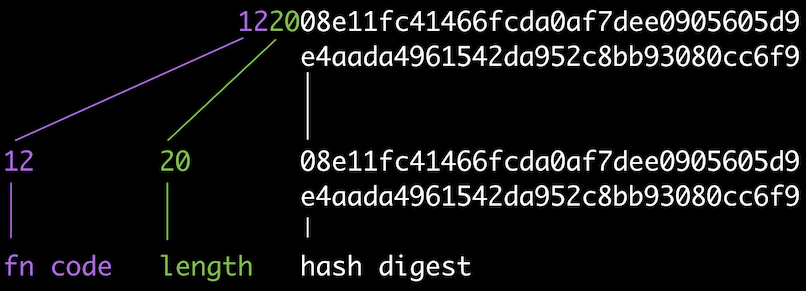
\includegraphics[width=10cm]{images/multihash.jpg}
    \caption{Anatomy of IPFS Multihash\protect\footnotemark}
    \label{img:anatomy-of-ipfs-multihash}
\end{figure}

\footnotetext{\url{https://github.com/multiformats/multihash}}

\newpage
\begin{figure}[H]
    \lstinputlisting[language=Solidity]{code-snippets/IPFSStorage.sol}
    \caption{Contract for transaction cost alanysis}
    \label{code:ipfs-storage}
\end{figure}


The contract defines four different methods for storing an IPFS multihash. Table \ref{tab:transaction-gas-cost-analysis} illustrates the gas costs for the different methods. As shown in these examples, the gas prices can be reduced by more than 70\% when storing an IPFS CID in the logs with data types of distinct length.

\begin{table}[ht]
\centering
\begin{tabular}{|c|c|c|c|c|c|}
\hline
\textbf{Method} & \textbf{Storage} & \textbf{Data Type} & \textbf{Gas Used} & \textbf{Price ETH} & \textbf{Price USD} \\ \hline
1               & contract         & string             & 86163             & 0.003              & 1.11               \\ \hline
2               & contract         & bytes              & 69848             & 0.002              & 0.90               \\ \hline
3               & log              & string             & 27675             & 0.001              & 0.35               \\ \hline
4               & log              & bytes              & 25841             & 0.001              & 0.33               \\ \hline
\end{tabular}
\caption{Transaction Gas Cost Analysis}
\label{tab:transaction-gas-cost-analysis}
\end{table}

\subsection{Correctness}
Evaluating the correctness of the contracts is done with a collection of tests. In total more than 90 automated integration tests are present. With this testing suite inconsistencies can be located quickly if updates are made to the contracts. 

\subsection{Discussion}
%connection all the point made in the evaluation
As shown in the gas price analysis, a new event is expensive to deploy but creating ticket types and minting new tickets is around 1 USD per ticket and type. However, the main benefit from this design is that the host and the guests must sign transactions as seldom as possible. Multiple non-fungible tickets of different types can be minted within the same transaction. This concept is applied to all the transactions in the ticket distribution, presale, as well as the aftermarket. One can create multiple presales with one transaction. Also, it is possible to create a buy order for multiple fungible as well as non-fungible types within a single transaction. Thus, the user experience is more like a traditional application where a customer only has to sign a transaction when the shopping cart is checked out.

The functionality of using other currencies such as stable coins are integrated in the contract by default. Every value transfer on the contract will be made in the selected currency by the event host. Transactions become slightly more expensive as shown in Table \ref{tab:gas-cost-buying-ticket-types-with-erc20} and require an additional approval transaction in the ERC20 contract. However, it enables the host and guests to transact with less volatile currencies. 

Solidity limits the size of a contract to 24KB. \cite{solidity-contract-size}. By encapsulating common functionality, data structures and constants into a shared library, the contract size is kept under this threshold. As explained in Section \ref{subsection:event-log-vs-public-getters}, the contract size can be reduced by either only using public getters or only the event log for accessing data. However, new features may increase the contract size such that it may no longer be deployed. In such a scenario, it could make sense to outsource the aftermarket functionality to a separate contract where one contract could manage the aftermarkets of all events.

Gas prices have risen by a factor of three since April 2020 \cite{ethereum-gas-price-chart}. Building a second layer solution was considered to lower the transaction fees. However, all layer two solutions in the Ethereum ecosystem such as Plasma \cite{plasma}, zkRollup \cite{zkrollup}, Optimistic Rollup \cite{optimistic-rollup} require the user to first deposit some cryptocurrency in the child chain. This deposit transaction is made on the main chain and thus, gas costs add up to a similar price as directly buying a ticket from the event SC. Since these coins are locked up in the child chain, users cannot use them outside of the child chain and would not be willing to deposit more than needed to buy tickets for one event. A second layer solution can make sense if tickets are invalidated on-chain or the ownership of a ticket is transferred multiple times. Otherwise, there is no radical benefit for this application using a second layer solution. 
